\chapter{Introducción}
\label{ch:introduction}

El \textit{skeleton} fue propuesto por Harry Blum en 1967 como una manera de capturar lo esencial de la forma de una figura biológica \cite{Blum:1967}. A diferencia de otros estímulos visuales como el color, la intensidad luminosa o el movimiento, Blum observó que el estudio de la forma habría estado sesgado por la geometría de las figuras. Las formas de figuras complejas, comunes en biología, casi no eran materia de estudio debido a la falta de herramientas para transformarlas en una combinación de componentes más simples. Blum postuló que la unión de los ejes medios, que más tarde sería llamada \textit{skeleton} \cite{hilitch1969linear}, podría haber sido la herramienta necesaria. Dada una figura, Blum define su \textit{skeleton} como una estructura delgada y centrada, geométrica y topológicamente expresiva.

\begin{figure}[ht]\centering
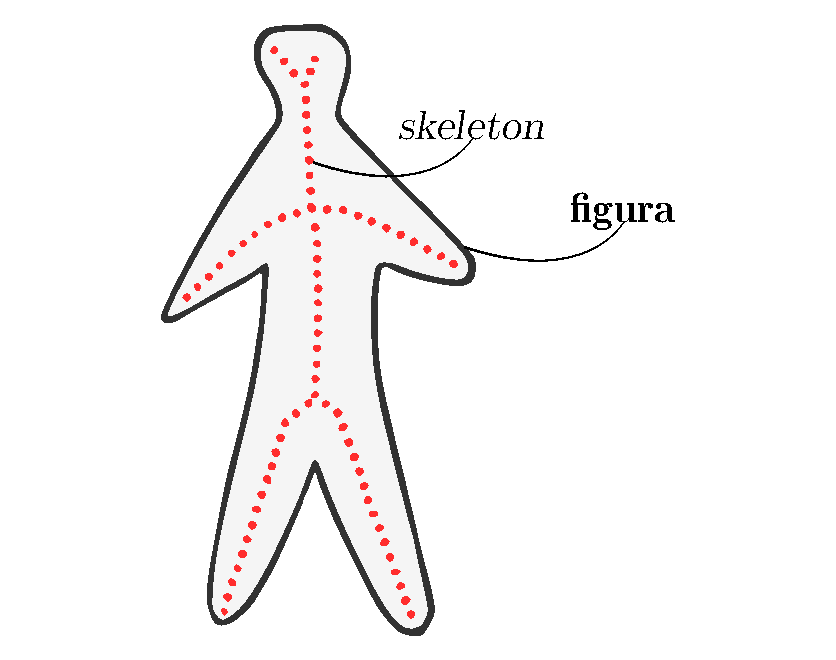
\includegraphics[width=0.5\linewidth]{images/blum}
\caption{Diagrama del \textit{skeleton} de una figura antropomórfica, como aparece en el artículo original de Blum \cite{Blum:1967}}
\label{fig:blum}
\end{figure}

Cincuenta años mas tarde, el \textit{skeleton} de Blum se ha convertido en uno de los descriptores de figuras más usados \cite{sobiecki2013qualitative}. La operación de calcular el \textit{skeleton} juega un rol central en muchas aplicaciones que involucran la búsqueda, manipulación, análisis o compresión de figuras en el computador, en áreas que van mucho más allá de la biología \cite{Saha2015}. La operación de calcular el \textit{skeleton} es también el foco de esta tesis. En principio, interesa responder la siguiente pregunta: ¿cuál es la mejor manera de llevar a cabo esta operación?

No obstante, existen dos dificultades importantes que impiden dar una respuesta rápida a la pregunta anterior.

\begin{enumerate}

\item Durante la extensa historia del \textit{skeleton} se han propuesto decenas de algoritmos para calcularlo. Siendo inviable comparar todos los métodos conocidos, es posible categorizarlos y seleccionar algoritmos representativos de cada clase. Sin embargo, las implementaciones de los algoritmos que calculan el \textit{skeleton} muy rara vez acompañan a sus publicaciones \cite{sobiecki2014comparison}.

\item No existe un consenso para la definición del \textit{skeleton}. Es más, existen aplicaciones donde calcular un \textit{skeleton} demasiado ajustado a alguna definición puede ser perjudicial \cite{cornea2007curve}. Esto significa que cualquier comparación entre estos algoritmos debe plantearse en cuanto a las restricciones y objetivos de alguna aplicación en particular \cite{Saha2015}.

\end{enumerate}

En consideración con lo anterior, este trabajo de tesis se divide en dos partes. La primera parte consiste en implementar algoritmos representativos de las distintas maneras que se han propuesto para calcular el \textit{skeleton}. Luego viene la parte de comparar los \textit{skeletons} calculados por estos algoritmos. Los datos (las figuras cuyo \textit{skeleton} se quiere calcular) y la justificación para la comparación propuesta están ligados a una aplicación muy similar a la originalmente visionada por Blum. Interesa evaluar los \textit{skeletons} calculados de acuerdo a métricas relevantes para la cuantificación de imágenes de figuras vivas microscópicas. En definitiva, la pregunta que busca responder esta tesis queda reformulada, a grandes rasgos, como sigue: ¿Qué clase de algoritmos para calcular el \textit{skeleton} es mejor para ciertas aplicaciones de biología?

\begin{figure}[ht]\centering
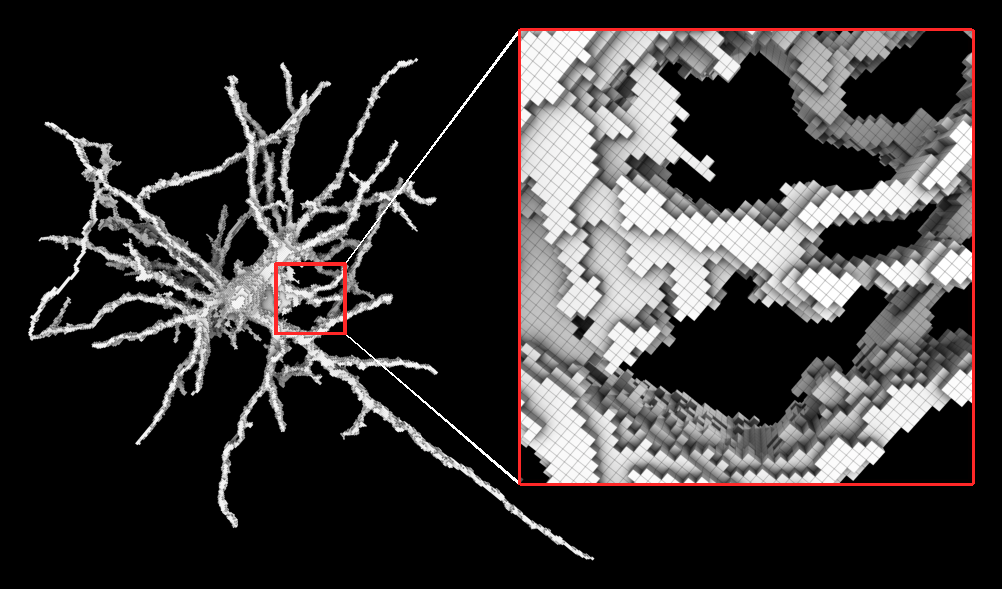
\includegraphics[width=1\linewidth]{images/neuron_with_closeup}
\caption{Ejemplo de los datos}
\label{neuron_with_closeup}
\end{figure}

El resto de este capítulo introductorio busca precisar lo señalado hasta este punto. Se revisan distintas maneras de definir el \textit{skeleton} de figuras 2D y 3D. Se detallan las propiedades del \textit{skeleton} de acuerdo a la literatura, dando ejemplos de aplicaciones donde satisfacer estas propiedades puede ser contraproducente. Finalmente, se explica la clasificación usada para seleccionar los algoritmos representativos implementados. La aplicación en biología mencionada se detalla en el Capítulo \ref{ch:results}.

\section{Definiciones del \textit{skeleton}}

En la literatura es posible encontrar por lo menos cuatro definiciones formales para el \textit{skeleton} \cite{tagliasacchi20163d}. En esta sección se detallan las dos definiciones más populares \cite{cornea2005computing}, que al mismo tiempo son las más relevantes para este trabajo.

\subsection{El \textit{skeleton} a partir de la metáfora del incendio}
\label{ssec:grassfire}

La metáfora del incendio de Blum \cite{Blum:1967} dice que el \textit{skeleton} de un objeto se puede obtener encendiéndole fuego a toda su frontera simultáneamente. Luego, se asume que los frentes de llamas se propagan a una velocidad constante hacia el interior del objeto. Una vez que el fuego ha alcanzado todo el objeto, el \textit{skeleton} queda formado en los lugares donde dos frentes distintos se encontraron. En otras palabras, el \textit{skeleton} corresponde a los puntos de extinción, donde el fuego no pudo seguir avanzando por haberse encontrado consigo mismo. Estos puntos se conocen hoy en día como \textit{puntos de choque} \cite{leymarie2003three}. La Figura \ref{fig:horseonfire} ilustra esta definición para una imagen 2D y la Figura \ref{fig:fireinthehorse} la muestra en una imagen volumétrica 3D.
\\\\
\begin{figure}[ht]\centering
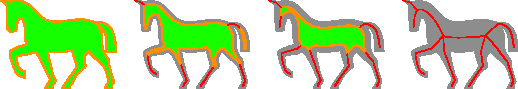
\includegraphics[width=0.9\linewidth]{images/horseonfire}
\caption{Progresión del incendio de Blum en una imagen 2D}.
\label{fig:horseonfire}
\end{figure}

\begin{figure}[ht]\centering
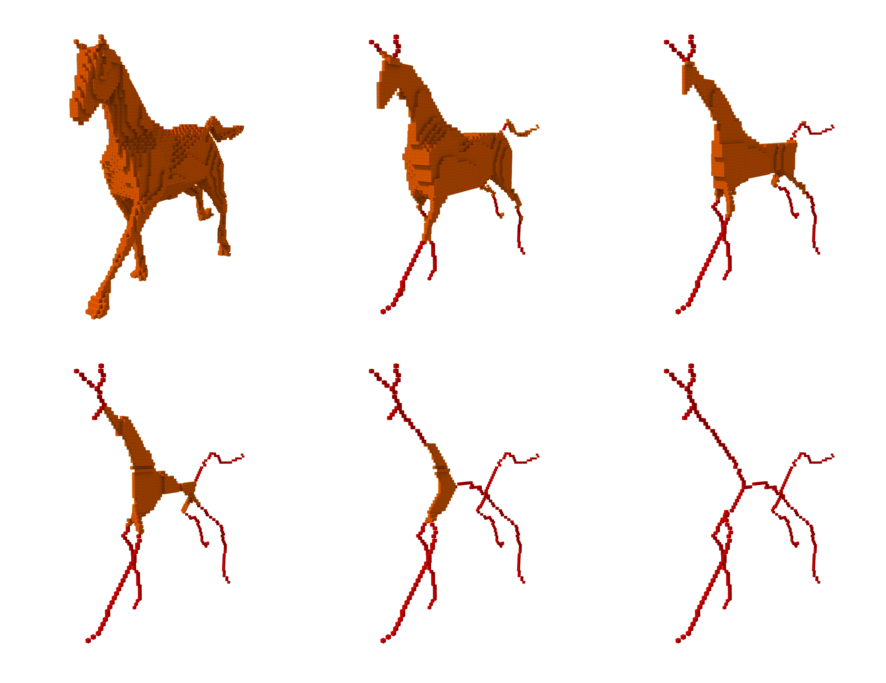
\includegraphics[width=0.9\linewidth]{images/fire_in_the_horse}
\caption{Progresión del incendio de Blum en un volumen de vóxeles}.
\label{fig:fireinthehorse}
\end{figure}

La propagación del fuego desde el borde de la figura es isotrópica, pudiendo ser descrita formalmente mediante la ecuación
\begin{equation} \label{eq:curve_evol}
\frac{\partial{\boldsymbol{C}(t)}}{\partial{t}} = f\boldsymbol{n},
\end{equation}
donde $\boldsymbol{C}(t)$ representa el borde de la figura a lo largo del tiempo, $f$ la velocidad constante de propagación y $\boldsymbol{n}$ la normal interior. Encontrar el \textit{skeleton} según esta definición significa detectar los puntos de choque de esta ecuación.

En este trabajo de tesis se implementaron dos algoritmos que en alguna medida se basan en esta definición. Estos son el algoritmo de adelgazamiento del Capítulo \ref{ch:palagyi} y el algoritmo de detección de singularidades del Capítulo \ref{ch:siddiqi}. En particular, el algoritmo del Capítulo \ref{ch:siddiqi} se fundamenta en un desarrollo formal de la ecuación anterior.

\subsection{El \textit{skeleton} como lugar geométrico}

La segunda definición más común para el \textit{skeleton} también aparece esbozada en el artículo de Blum. En él, Blum nota que cada punto de choque $p$, al ser el lugar de encuentro de frentes de propagación diferentes, siempre es equidistante a por lo menos dos puntos distintos del borde de la figura, que a la vez son los puntos del borde de la figura más cercanos a $p$. Es decir que, dado un punto $p$ del interior de la figura, $p$ es un punto del \textit{skeleton} si existen dos puntos $q$ y $r$ en el  borde $\boldsymbol{C}$ de la figura tales que

\begin{enumerate}
\item $\lVert q - p \rVert = \lVert r - p \rVert = \mathcal{R}_p$ y
\item $\nexists s \in \boldsymbol{C} \mid \lVert s - p \rVert < \mathcal{R}_p$,
\end{enumerate}

\noindent
para algún $\mathcal{R}_p > 0$.

Entonces, para todo punto $p$ del \textit{skeleton} es posible definir un esfera (o un disco en el caso 2D) con centro $p$ y radio $\mathcal{R}_p$ completamente inscrita en la figura. Además, el borde de esta esfera comparte por lo menos dos puntos con el borde de la figura. Se dice que una esfera con estas propiedades es una \textit{esfera maximal inscrita} en la figura.

El \textit{skeleton} de una figura queda definido, por lo tanto, como el lugar geométrico de los centros de las esferas maximales inscritas en la figura. El problema de calcular el \textit{skeleton} se traduce en la detección de estos centros. La Figura \ref{fig:rect_cbm} muestra un punto del \textit{skeleton} de un paralelepípedo y su correspondiente esfera maximal.

\begin{figure}[ht]\centering
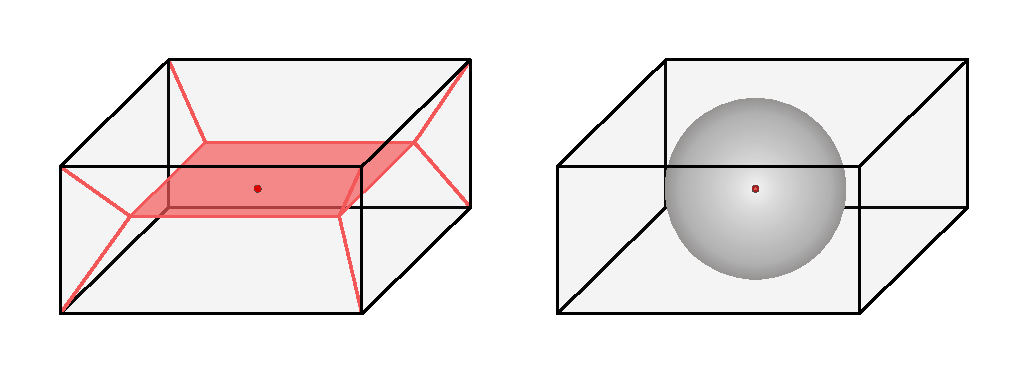
\includegraphics[width=0.9\linewidth]{images/rect_cbm}
\caption{Centro de una esfera maximal inscrita}
\label{fig:rect_cbm}
\end{figure}

Detectar los centros de las esferas maximales es excesivamente costoso usando métricas exactas \cite{borgefors1996digital}. El primer paso del algoritmo del Capítulo \ref{ch:arcelli}, basado parcialmente en esta definición, usa una métrica sencilla para detectar estos centros de manera aproximada.

\section{El \textit{skeleton} curvilíneo y el \textit{skeleton} de superficie}

El \textit{skeleton} de una figura 2D está siempre formado por curvas 1D. En cambio, para figuras 3D es posible definir dos tipos de \textit{skeleton}. En primer lugar está el \textit{skeleton de superficie}, que además de curvas 1D puede contener parches de superficie 2D. El \textit{skeleton} de superficie preserva la geometría general de la figura original. Esto en el sentido de que, tomando algunas consideraciones menores, la figura original podría recuperarse íntegramente a partir de su \textit{skeleton} de superficie \cite{borgefors1999computing}.

Sin embargo, salvo en aplicaciones donde interesa comprimir o reconstruir las figuras 3D originales, el \textit{skeleton} de superficie no es de mucha utilidad práctica. Su estructura es difícil de manipular y la presencia de parches de superficie lo vuelve inadecuado para muchas aplicaciones \cite{huang2013l1}. El \textit{skeleton curvilíneo}, una simplificación  del \textit{skeleton} de superficie formada exclusivamente por curvas 1D, es de mayor utilidad práctica. La Figura \ref{fig:surface_skel} muestra los \textit{skeletons} de superficie y curvilíneo para una volumen 3D.

\begin{figure}[H]\centering
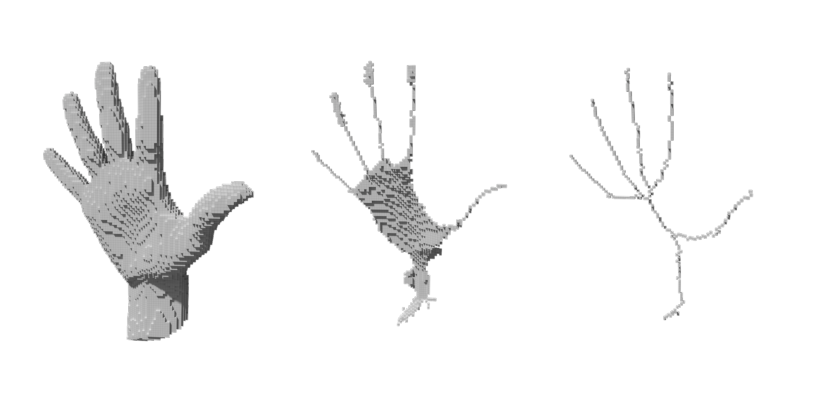
\includegraphics[width=1.0\linewidth]{images/surface_skel}
\caption{Una figura 3D y sus \textit{skeletons} de superficie y curvilíneo}
\label{fig:surface_skel}
\end{figure}

Existen algoritmos que calculan el \textit{skeleton} de superficie, otros que calculan el \textit{skeleton} curvilíneo a partir del \textit{skeleton} de superficie y otros que calculan directamente el \textit{skeleton} curvilíneo. La mayoría de los algoritmos basan su diseño en alguna de las definiciones anteriores, independientemente al tipo de \textit{skeleton} calculado.

Por otra parte, el \textit{skeleton} curvilíneo es el descriptor requerido en las aplicaciones que motivan esta tesis. Entonces, todos los algoritmos implementados para esta tesis calculan el \textit{skeleton} curvilíneo. Los algoritmos de los Capítulos \ref{ch:palagyi} y \ref{ch:siddiqi} calculan el \textit{skeleton} curvilíneo directamente y el algoritmo del Capíulo \ref{ch:arcelli} lo calcula a partir del \textit{skeleton} de superficie.

En adelante, salvo cuando se indique algo distinto, la palabra \textit{skeleton} se usará para referirse al \textit{skeleton} curvilíneo en el caso 3D.

\section{Propiedades del \textit{skeleton}} \label{sec:skelprops}

Las distintas definiciones del \textit{skeleton} son equivalentes en teoría; es decir, en conjunto sugieren la existencia de un \textit{skeleton} analítico. Sin embargo, llevar las definiciones a la práctica significa crear algoritmos fundamentalmente distintos entre sí. Como se comprobará a lo largo de esta tesis, dos algoritmos que adopten la misma definición como punto de partida pueden producir \textit{skeletons} muy diferentes. Las figuras son representadas de manera discreta en el computador, lo cual introduce gran variabilidad en los cálculos \cite{reniers2008computing}.

De lo anterior se desprende que las definiciones del \textit{skeleton} no son suficientes para verificar el resultado de un algoritmo de cálculo del \textit{skeleton}. Más bien solamente sirven como base para el diseño de un algoritmo.

Esto ha llevado a definir las siguientes propiedades fundamentales que debería satisfacer el \textit{skeleton} calculado por cualquier algoritmo. Observar el cumplimiento de estas propiedades sirve como una validación cualitativa de los resultados de un algoritmo. Dado que algunas de las siguientes propiedades son contradictorias entre sí, algoritmos diferentes las satisfacen en distinta medida. Al mismo tiempo, aplicaciones diferentes favorecen algunas propiedades por sobre otras. Las propiedades más comúnmente encontradas \cite{cornea2007curve,tagliasacchi2012mean} se detallan a continuación.

\subsection{Homotopía}

El \textit{skeleton} debe tener la misma topología que la figura a partir de la cual es calculado. Esto significa que el cálculo del \textit{skeleton} debe preservar el número de componentes conexas en 2D y además el número de túneles en 3D \cite{Lieutier20041029}. Estos conceptos se profundizan en el Capítulo \ref{ch:defs}.

\subsection{Invariancia}

El cálculo del \textit{skeleton} debe ser resistente a transformaciones isométricas. Por ejemplo, calcular el \textit{skeleton} de una figura y luego rotar el \textit{skeleton} calculado debería dar el mismo resultado que primero rotar la figura y luego calcular su \textit{skeleton}.

\subsection{Centralidad}

El \textit{skeleton} debe estar centrado en la figura original. Es decir, debe quedar ubicado en los centros de los ejes y planos de simetría de las partes de la figura.

\subsection{Delgadez}

El \textit{skeleton} de una figura de $n$ dimensiones debe ser una figura cuyas partes tienen a lo más $n-1$ dimensiones. El \textit{skeleton} se puede definir para un número de dimensiones arbitrario \cite{Lieutier20041029}, pero para esta tesis, puesto que concierne figuras representadas visualmente en el computador, $n$ vale 2 o 3. Entonces, el \textit{skeleton} de una figura 2D debe una unión de curvas y el \textit{skeleton} de una figura 3D puede estar formado por curvas y parches de superficie (aunque, como se señaló anteriormente, para esta tesis interesa que solo sean curvas).

\subsection{Suavidad}

Algunas aplicaciones requieren que el \textit{skeleton} no tenga saltos bruscos \cite{wan2002automatic}. En teoría, el \textit{skeleton} debería estar formado por curvas de clase $\mathcal{C}^2$, es decir, curvas continuas hasta su segunda derivada. Sin embargo, suavizar el \textit{skeleton} en este sentido va siempre en detrimento de la centralidad.

\subsection{Robustez}

El cálculo del \textit{skeleton} debería ser resistente a perturbaciones pequeñas en el borde de las figuras. En otras palabras, el \textit{skeleton} de una figura debería ser parecido al \textit{skeleton} de esa misma figura con algo de ruido. Esta propiedad es deseable, puesto que un \textit{skeleton} estricto es muy sensible al ruido, reduciendo su valor expresivo. Sin embargo, la robustez siempre se gana a costa de perder reconstructibilidad.

\subsection{Reconstructibilidad}

El cálculo del \textit{skeleton} debería ser en teoría reversible. La figura original deberia poderse reconstruir a partir de los puntos del \textit{skeleton} y los radios de las esferas maximales correspondientes. Esto es particularmente deseable en aplicaciones donde el \textit{skeleton} se usa para la compresión de datos \cite{lien2007skeleton,huang1990astronomical}.

\section{Clases de algoritmos}

En principio, los algoritmos de cálculo del \textit{skeleton} pueden dividirse en dos, según el tipo de dato que reciben como entrada. Están los algoritmos que operan sobre mallas geométricas y los que operan sobre volúmenes de vóxeles. Para esta tesis se implementaron exclusivamente algoritmos que operan sobre volúmenes de vóxeles. Cada algoritmo implementado es representativo de alguna de las tres clases que se encuentran en la literatura \cite{cornea2007curve, Saha2015, tagliasacchi20163d}.

\subsection{Algoritmos de adelgazamiento}

El enfoque más intuitivo y divulgado para este problema usa la definición de punto simple de Morgenthaler \cite{lam1992thinning,university1981three,saha1994topology} para erosionar progresivamente el borde de un objeto de vóxeles, capa por capa, hasta lograr el ancho unitario \cite{hilitch1969linear,lobregt1980three,arcelli1985width,borgefors1999computing}. Abordar el problema de esta forma es cercano a simular la transformada del incendio propuesta por Blum. Con el fin de reducir el costo computacional, también se ha propuesto hacer la eliminación de vóxeles en paralelo \cite{gong1990simple,saha1997new,palagyi1999parallel}.

En el Capítulo \ref{ch:palagyi} se detalla la implementación del algoritmo de adelgazamiento paralelo presentado en \cite{palagyi1999parallel}.

\subsection{Algoritmos basados en la distancia}

Una manera alternativa de adelgazar la figura es incorporar en el cálculo información de la distancia de cada vóxel al borde \cite{pudney1998distance}. Siguiendo este enfoque, existen varios algoritmos que buscan cimas en la transformada de distancia para centrar el \textit{skeleton}. Esto equivale a encontrar los centros de las esferas maximales \cite{di1994well,pudney1998distance,perchet2004advanced}. También se han propuesto otros campos basados en la distancia, de orden escalar \cite{ahuja1997shape,go1997extraction} y vectorial \cite{cornea2005computing,hassouna2009variational,short2013spatial}.

Por lo general estos algoritmos deben calcular primero el \textit{skeleton} de superficie para el caso 3D. Luego, el \textit{skeleton} curvilíneo es calculado como un subconjunto centrado en el \textit{skeleton} de superficie. Esto les permite un mayor grado de centralidad en comparación con las demás clases de algoritmos \cite{tagliasacchi2012mean}. El algoritmo de Arcelli et al \cite{arcelli2011distance}, cuya implementación es detallada en el Capítulo \ref{ch:siddiqi}, es el representante de esta categoría.

\subsection{Algoritmos de evolución continua de curvas}

Otros algoritmos se basan en el principio de propagación de curvas, que consiste en deformar continuamente los contornos hacia el interior del objeto. Estrictamente, este proceso podría consistir en modelar de alguna manera la evolución de los contornos usando la ecuación \ref{eq:curve_evol}. En esta simulación, el \textit{skeleton} quedaría formado en los puntos de colisión de bordes opuestos \cite{kimmel1995skeletonization,leymarie2003three}. El libro de Siddiqi et al. \cite{siddiqi2008medial} proporciona una buena recopilación de algoritmos de esta categoría.

Para esta tesis se implementó el algoritmo de Siddiqi et al. \cite{siddiqi2002hamilton}. Este algoritmo no consiste en una simulación, sino que usa un desarrollo matemático para reducir el problema significativamente. Los detalles se exponen en el Capítulo \ref{ch:siddiqi}.

\subsection{Algoritmos para representaciones geométricas}

Como se mencionó anteriormente, existen muchos algoritmos para calcular el \textit{skeleton} a partir de mallas geométricas. Ejemplos de esta aproximación son el uso de diagramas de Voronoi para extraer \textit{skeletons} 2D \cite{ogniewicz1992voronoi,ogniewicz1995hierarchic,liu2012generation} y 3D \cite{sherbrooke1996algorithm,dey2004approximating}, colapso de mallas geométricas \cite{au2008skeleton,janoos2009robust} y otras operaciones de centralidad \cite{bucksch2010skeltre,huang2013l1}.

Aunque no se implementó un representante de esta clase de algoritmos para esta tesis, se incluye en la comparación la implementación del algoritmo de Au et. al \cite{au2008skeleton} fruto de los trabajos de memoria de Liliana Alcayaga e Iván Rojas \cite{Alcayaga2012, rojas2014optimizacion}.

\vspace{5mm}

La clasificación anterior no es estricta, puesto que varios algoritmos rescatan elementos de más de una clase. Por ejemplo, el algoritmo del Capítulo \ref{ch:arcelli} usa adelgazamiento para asegurar la delgadez del \textit{skeleton}. Sin embargo, el objetivo de este trabajo es proponer para una evaluación cuantitativa de propósito general. Con esto en mente, implementar un método de cada clase busca ilustrar los alcances generales de las métricas de comparación propuestas.


\section{Estructura de esta tesis}

El siguiente capítulo presenta algunos conceptos básicos de topología digital, necesarios para comprender los capítulos posteriores. Los tres capítulos que lo preceden describen cada uno un algoritmo de cálculo del \textit{skeleton} implementado. Cada uno de estos capítulos sigue la misma estructura. Primero se exponen algunos fundamentos teóricos para luego dar paso al detalle de la implementación. Estos algoritmos fueron programados en el lenguaje MATLAB. Por completitud se incluye en el Capítulo \ref{ch:results} una descripción del algoritmo para representaciones geométricas anteriormente mencionado.
